%!TEX root = edance.tex
%%%%%%%%%%%%%%%%
%   CHAPTER 4  %
%%%%%%%%%%%%%%%%
\chapter{IC Resistors and Capacitors and Electrostatics}
\label{ch:ch04_ic_tech}
\graphicspath{{./figs_ic_tech/}}
%%%%%%%%%%%%%%%%%%%%%%%%%%%%%%%%%%%%%%%%%%%%%%%%%%%%%%%%%%%%%%%%%%%%%%%%%%%%%%%%%%%%%%%%
%%%%%%%%%%%%%%%%%%%%%%%%%%%%%%%%%%%%%%%%%%%%%%%%%%%%%%%%%%%%%%%%%%%%%%%%%%%%%%%%%%%%%%%%
%                                   SECTION 4.1                                        %
%%%%%%%%%%%%%%%%%%%%%%%%%%%%%%%%%%%%%%%%%%%%%%%%%%%%%%%%%%%%%%%%%%%%%%%%%%%%%%%%%%%%%%%%
%%%%%%%%%%%%%%%%%%%%%%%%%%%%%%%%%%%%%%%%%%%%%%%%%%%%%%%%%%%%%%%%%%%%%%%%%%%%%%%%%%%%%%%%
\section{Chapter Preview}
In this short chapter we discuss integrated circuit device fabrication, in particular fabrication of resistors.  The fabrication steps also apply to capacitors, diodes and transistors, devices which we will cover in the following chapters.  Next, we will review electrostatics, a topic of integral importance in the next chapter.  Readers familiar with electrostatics can skip or skim these sections.  Finally, we discuss capacitors and in particular non-linear capacitors, or devices that have a non-linear charge-voltage characteristic.  We shall see in the next two chapters that reverse-biased diodes are essentially non-linear capacitors.
%%%%%%%%%%%%%%%%%%%%%%%%%%%%%%%%%%%%%%%%%%%%%%%%%%%%%%%%%%%%%%%%%%%%%%%%%%%%%%%%%%%%%%%%
%%%%%%%%%%%%%%%%%%%%%%%%%%%%%%%%%%%%%%%%%%%%%%%%%%%%%%%%%%%%%%%%%%%%%%%%%%%%%%%%%%%%%%%%
%                                   SECTION 4.2                                        %
%%%%%%%%%%%%%%%%%%%%%%%%%%%%%%%%%%%%%%%%%%%%%%%%%%%%%%%%%%%%%%%%%%%%%%%%%%%%%%%%%%%%%%%%
%%%%%%%%%%%%%%%%%%%%%%%%%%%%%%%%%%%%%%%%%%%%%%%%%%%%%%%%%%%%%%%%%%%%%%%%%%%%%%%%%%%%%%%%
\section{IC Fabrication: Si Substrate}
For most semiconductors, a pure \textbf{ingot}\index{Ingot} of a silicon ($Si$) crystal cut into thin wafers is the starting material for fabrication.  The $Si$ wafer is extremely pure ($\sim$1 part in a billion impurities).  As we learned in the last chapter, this level of purity is necessary in order selectively dope the semiconductor to alter its properties.  The Si crystal structure has a density of about $\num{5e22}$, and we typically dope regions of the substrate with doping levels ranging from  $10^{14}$ – $10^{18}$.  We want the unintentional dopants (impurities) to be about one to two orders of magnitude less dense $\sim$ $10^{12}$ in order to realize a high quality device.  

$Si$ wafers are polished to about $700\;\mu m$ thick with a mirror finish.  The $Si$ forms the substrate for the IC, and all the structures are built on the thin films on the top layer of the substrate.  
%%%%%%%%%%%%%%%%%%%%%%%%%%%%%%%%%%%%%%%%%%%%
%             SUBSECTION 4.2.1             %
%%%%%%%%%%%%%%%%%%%%%%%%%%%%%%%%%%%%%%%%%%%%
\subsection{IC Fabrication: Oxide}
$Si$ has a native oxide, $SiO_2$.  $SiO_2$ (Quartz) is extremely stable and very convenient for fabrication.  It is an insulator, so it can be used for house interconnection on top of the substrate (wires interconnecting various devices for example).  It can also be used for selective doping by using $SiO_2$ to block doping in regions where we don't want to dope, and by chemically etching openings or windows using \textbf{photolithography}\index{Photolithography} (described below) to dope regions.  These openings allow ion implantation into selected regions, and $SiO_2$ can block ion implantation in other areas.
%%%%%%%%%%%%%%%%%%%%%%%%%%%%%%%%%%%%%%%%%%%%
%             SUBSECTION 4.2.2             %
%%%%%%%%%%%%%%%%%%%%%%%%%%%%%%%%%%%%%%%%%%%%
\subsection{IC Fabrication: Ion Implantation}
%%%%%%%%%%%%%%%%%%%%%%%%%%%%%%%%%%%%%%%%%%%%
%                 FIGURE                   %
%%%%%%%%%%%%%%%%%%%%%%%%%%%%%%%%%%%%%%%%%%%%
\begin{figure}[tb]
\centering
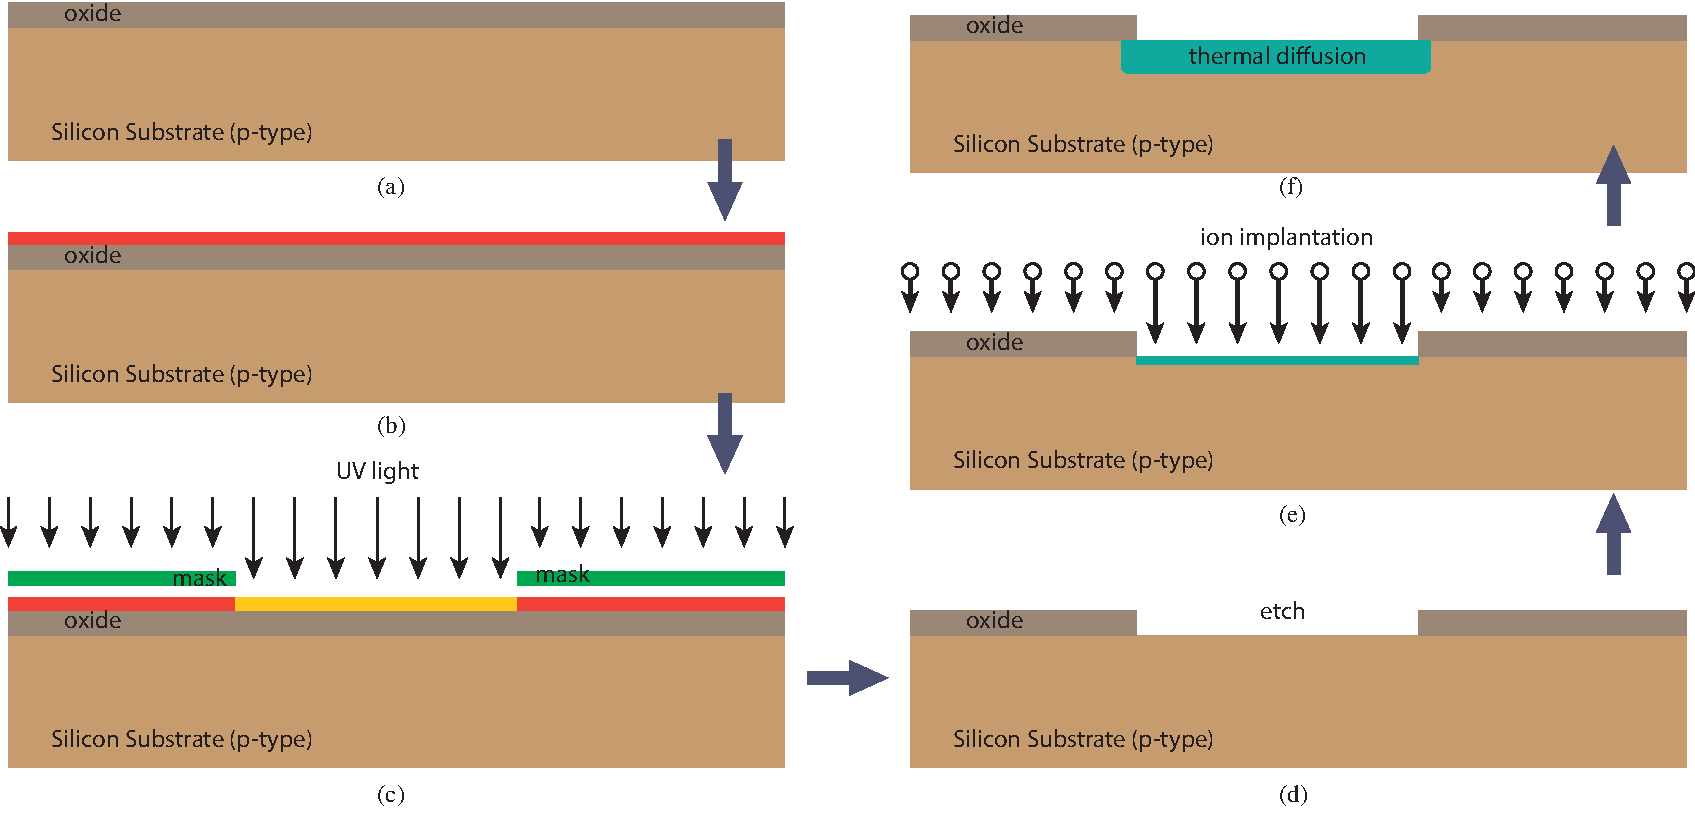
\includegraphics[width=\columnwidth]{process_steps}
\caption{The fabrication steps in a typical photolithography process to create a diffusion region in the silicon substrate.  The steps include (a) oxide growth and (b) deposition of a photoresist over the surface; (c) selective exposure to UV using a mask; (d) chemical etching to wash away regions exposed to UV; (e) ion-implantation; (f) diffusion to allow implants to diffuse into the structure.} \label{fig:mod2-2_ICtech_sld_4}
\end{figure}
%%%%%%%%%%%%%%%%%%%%%%%%%%%%%%%%%%%%%%%%%%%%
The steps involved in ion implantation are shown in \emph{Fig.~\ref{fig:mod2-2_ICtech_sld_4}}.  We start with a Si substrate.  It is usually pre-doped to be \emph{P}-type, but this depends on the details of the process.  We grow a layer of oxide (thermally) by heating the substrate and flowing oxygen onto the surface.  Next, we cover the surface with \textbf{photoresist}\index{Photoresist}, a material that changes its chemical properties based on exposure to light.  We use photolithography to selectively expose regions of the photoresist using a UV source and a lithography mask.  Next, we chemically etch (using an acid such as $HF$)  the surface, removing areas exposed to UV light.\footnote{This kind of photoresist is "positive" because exposure to light chemically alters the material so that it reacts with an acid. There's also  "negative" photoresist materials too that don't react with the acid when exposed.}  Finally, we introduce ion implantation (\emph{N}-type), whereby we inject dopants onto the entire surface of the wafer.  Regions with the $SiO_2$ are protected and block the ions, whereas the window openings allow the ions to be implanted into the silicon substrate.  Next, a higher temperature is used to allow the dopants to diffuse into the substrate and to form bonds with the silicon crystal.
\newpage
%%%%%%%%%%%%%%%%%%%%%%%%%%%%%%%%%%%%%%%%%%%%%%%%%%%%%%%%%%%%%%%%%%%%%%%%%%%%%%%%%%%%%%%%
%%%%%%%%%%%%%%%%%%%%%%%%%%%%%%%%%%%%%%%%%%%%%%%%%%%%%%%%%%%%%%%%%%%%%%%%%%%%%%%%%%%%%%%%
%                                   SECTION 4.3                                        %
%%%%%%%%%%%%%%%%%%%%%%%%%%%%%%%%%%%%%%%%%%%%%%%%%%%%%%%%%%%%%%%%%%%%%%%%%%%%%%%%%%%%%%%%
%%%%%%%%%%%%%%%%%%%%%%%%%%%%%%%%%%%%%%%%%%%%%%%%%%%%%%%%%%%%%%%%%%%%%%%%%%%%%%%%%%%%%%%%
\section{IC Resistors}
%%%%%%%%%%%%%%%%%%%%%%%%%%%%%%%%%%%%%%%%%%%%
%             SUBSECTION 4.3.1             %
%%%%%%%%%%%%%%%%%%%%%%%%%%%%%%%%%%%%%%%%%%%%
\subsection{“Diffusion” Resistor}
%%%%%%%%%%%%%%%%%%%%%%%%%%%%%%%%%%%%%%%%%%%%
%                 FIGURE                   %
%%%%%%%%%%%%%%%%%%%%%%%%%%%%%%%%%%%%%%%%%%%%
\begin{figure}[tb]
\centering
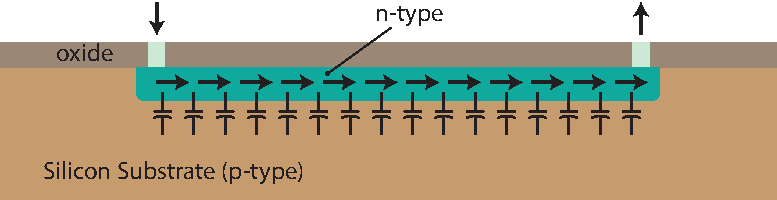
\includegraphics[width=.7\columnwidth]{diff_resistor}
\caption{Cross-section of an IC diffusion resistors in a \emph{P}-type region is made with an \emph{N}-type diffusion region and contacts.}
\label{fig:mod2-2_ICtech_sld_5}
\end{figure}
%%%%%%%%%%%%%%%%%%%%%%%%%%%%%%%%%%%%%%%%%%%%
Using ion implantation and diffusion, we can create a so-called \textbf{"diffusion resistor"}\index{Diffusion resistor}, shown in \emph{Fig.~\ref{fig:mod2-2_ICtech_sld_5}}.  The thickness and dopant concentration of resistor is set by process steps, whereas the shape of the resistor is set by design (layout).   Metal contacts are connected to ends of the resistor.  You may be wondering why current would flow through a thin diffusion layer rather than through the silicon substrate, which is comparatively much larger (wider and thicker).  The reason is that the resistor is DC isolated from the substrate, and only high frequency AC currents can flow from the diffusion region into the substrate.  In other words, there is a distributed capacitor from the resistor to the substrate, which is usually connected to ground potential.  This happens because the diffusion region is \emph{N}-type and the substrate is \emph{P}-type.  This \textbf{$PN$-junction}\index{PN-junction} should be \textbf{reverse biased}\index{PN-junction!Reverse biased} at all times (meaning the diffusion resistor should never be biased at a negative potential with respect to the substrate).  We will learn the details of \emph{PN}-junctions in the next chapter.
%%%%%%%%%%%%%%%%%%%%%%%%%%%%%%%%%%%%%%%%%%%%
%             SUBSECTION 4.3.2             %
%%%%%%%%%%%%%%%%%%%%%%%%%%%%%%%%%%%%%%%%%%%%
\subsection{Poly Film Resistor}
%%%%%%%%%%%%%%%%%%%%%%%%%%%%%%%%%%%%%%%%%%%%
%                 FIGURE                   %
%%%%%%%%%%%%%%%%%%%%%%%%%%%%%%%%%%%%%%%%%%%%
\begin{figure}[tb]
\begin{center}
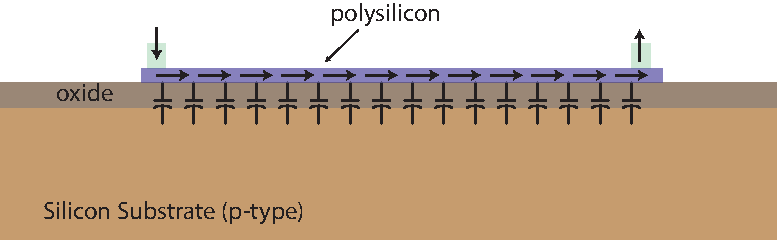
\includegraphics[width=.7\columnwidth]{poly_resistor}
\end{center}
\caption{Cross-section of a polysilicon resistor is made with a thin film of material on top of the oxide.}
\label{fig:mod2-2_ICtech_sld_6}
\end{figure}
%%%%%%%%%%%%%%%%%%%%%%%%%%%%%%%%%%%%%%%%%%%%
To lower any \textbf{parasitic capacitance}\index{Parasitic capacitance}, we should build the resistor further away from substrate, as shown in \emph{Fig.~\ref{fig:mod2-2_ICtech_sld_6}}. This is done by depositing a thin film of “poly” $Si$ (heavily doped) material on top of the oxide, rather than directly on the substrate.  This thin film resistor is not made of the crystalline form of silicon, but rather it is a \textbf{polycrystalline}\index{Polycrystalline} form, which is a material made with many fragments of crystals, of varying sizes and arranged in different orientations.   For our purposes, the material behaves similar to a crystal and we can model it as a doped semiconductor.  The process technology details set the thickness and resistance of this layer ( say $10\Omega/\Box$, see Section~\ref{sec:sheetR})
\newpage
%%%%%%%%%%%%%%%%%%%%%%%%%%%%%%%%%%%%%%%%%%%%
%             SUBSECTION 4.3.3             %
%%%%%%%%%%%%%%%%%%%%%%%%%%%%%%%%%%%%%%%%%%%%
\subsection{Ohm’s Law}
%%%%%%%%%%%%%%%%%%%%%%%%%%%%%%%%%%%%%%%%%%%%
%                 FIGURE                   %
%%%%%%%%%%%%%%%%%%%%%%%%%%%%%%%%%%%%%%%%%%%%
\begin{figure}[tb]
\centering
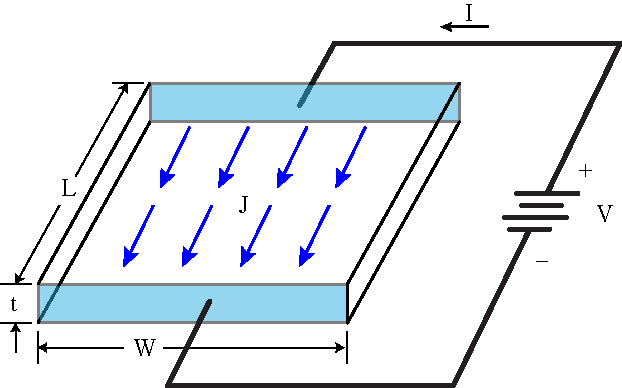
\includegraphics[width=.5\columnwidth]{ohms_law_slab}
\caption{A slab of silicon (or any material) forms a resistor and the current flows due to drift.  The fields inside the material arise due to the applied external voltage.}
\label{fig:ohms_law_slab}
\end{figure}
%%%%%%%%%%%%%%%%%%%%%%%%%%%%%%%%%%%%%%%%%%%%
With reference to \emph{Fig.~\ref{fig:ohms_law_slab}}, consider the current $I$ in terms of the current density $J$:
    \begin{equation*}
         I = J\,A = J\,t\,W = (\sigma \mathcal{E})\,t\,W
    \end{equation*}   
The voltage $V$ dropped across the resistor can be written in terms of electric field:  $E = V/L$.  Putting all of this together, we have:
    \begin{equation*} 
        I =  \left( \sigma\frac{V}{L} \right) t\,W = \left( \frac{\sigma t\,W} {L} \right)  V= \frac{1}{R} V
    \end{equation*}
This is nothing but Ohm's Law\index{Ohm's Law}, with the material resistance given by:
    \begin{align} 
        R &= \frac{L}{W}\,\frac{1}{{\sigma \,t}} &\textit{Material resistance} 
    \end{align}
%%%%%%%%%%%%%%%%%%%%%%%%%%%%%%%%%%%%%%%%%%%%
%             SUBSECTION 4.3.4             %
%%%%%%%%%%%%%%%%%%%%%%%%%%%%%%%%%%%%%%%%%%%%
\subsection{Sheet Resistance (\texorpdfstring{$R_{\Box}$}{})} \label{sec:sheetR}
The resistance of a rectangular slab of material can be written in a way as to distinguish process specific parameters (such as doping levels and material thickness) from layout (geometry) parameters, such as length and width: 
    \begin{align} 
        R &= \frac{resistivity}{thickness} = \frac{{\rho L}}{{Wt}} = \left( {\frac{\rho }{t}} \right)\left( {\frac{L}{W}} \right)
        = {R_{\Box}}\left( {\frac{L}{W}} \right) &\textit{Sheet resistance}
    \end{align}
Notice that $R_{\Box}$ is a convenient way to capture the process specific parameters.  Since IC resistors have a specified fixed thickness and resistivity – something not under the control of the circuit designer – we lump these parameters into a constant $R_{\Box}$.  This term is known as the \textbf{sheet resistance}\index{Sheet resistance}.  Even though it has units of resistance, or $\Omega$, we emphasize that it is a sheet resistance by the symbol $\Box$, since $R_{\Box}$ is the resistance of a square ($L = W$ implies $L/W = 1$).  
%%%%%%%%%%%%%%%%%%%%%%%%%%%%%%%%%%%%%%%%%%%%
%             SUBSECTION 4.3.5             %
%%%%%%%%%%%%%%%%%%%%%%%%%%%%%%%%%%%%%%%%%%%%
\subsection{Using Sheet Resistance (\texorpdfstring{$R_\Box$}{})}
Consider the ion-implanted (or “diffused”) IC resistor shown in \emph{Fig.~\ref{fig:diff_resistor_top}}.  We show both the cross-section and the top view.  To figure out the resistance, we just count the number of "squares" from end to end and multiply by $R_\Box$.  On the other hand, we know that there are regions where the current density $J$ "turns” or spreads, and so not all of square contains equal current.   Contact regions also have non-uniform current distribution as the current spreads out from a small via opening to the entire width of the resistor at one end, and then the inverse process occurs at the other end.  To account for the non-uniform current flow, we find that some simple rules of thumb can be applied.  As shown in \emph{Fig.~\ref{fig:dog_bone_squares}}, when turning corners, only about half (0.56 squares) of the metal contributes resistance, since some of the current will flow on the "inner track" and little current flows on the "outer track".  Likewise, when current spreads out from a via, only about 65\% of the region contributes resistance, and a good rule of thumb for "dog bone" layout resistors is to count the contact region as 0.65 squares.
%%%%%%%%%%%%%%%%%%%%%%%%%%%%%%%%%%%%%%%%%%%%
%                 FIGURE                   %
%%%%%%%%%%%%%%%%%%%%%%%%%%%%%%%%%%%%%%%%%%%%
\begin{figure}[tb]
\centering
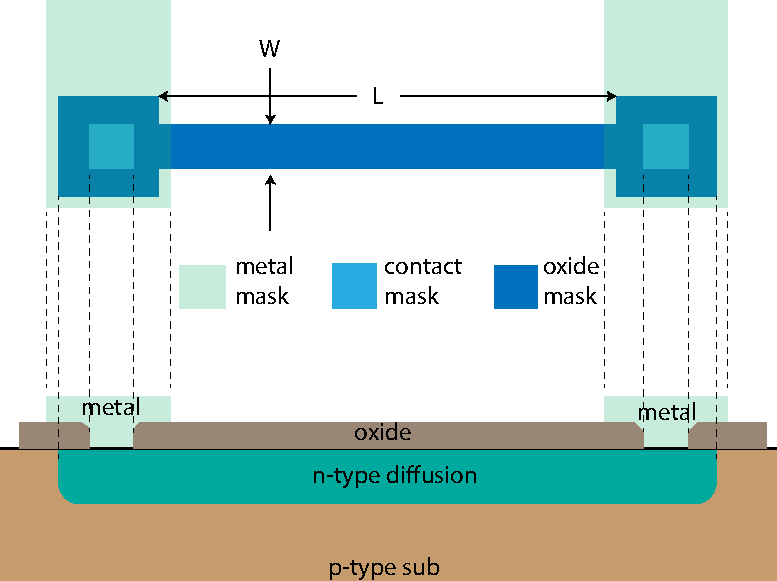
\includegraphics[width=.7\columnwidth]{diff_resistor_top}
\caption{Layout and cross section of a resistor using a "dog bone" layout to introduce contacts on either side which define the terminals of the resistor.}
\label{fig:diff_resistor_top}
\end{figure}
%%%%%%%%%%%%%%%%%%%%%%%%%%%%%%%%%%%%%%%%%%%%
%                 FIGURE                   %
%%%%%%%%%%%%%%%%%%%%%%%%%%%%%%%%%%%%%%%%%%%%
\begin{figure}[tb]
\centering
\begin{tabular}{ccc}
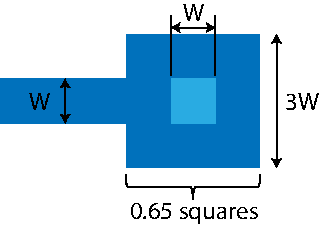
\includegraphics[width=.25\columnwidth]{dog_bone_squares} &
\hspace{2cm} &
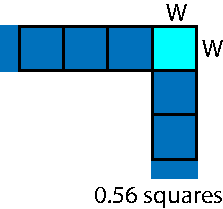
\includegraphics[width=.25\columnwidth]{corner_squares}\\
(a) & & (b)\\
\end{tabular}
\caption{(a) Due to non-uniform current flow, a contact region contributes approximately only 0.65 squares of resistance. (b) Similarly, current turning a corner only contributes 0.56 squares of resistance.}
\label{fig:dog_bone_squares}
\end{figure}
%%%%%%%%%%%%%%%%%%%%%%%%%%%%%%%%%%%%%%%%%%%%
\newpage
%%%%%%%%%%%%%%%%%%%%%%%%%%%%%%%%%%%%%%%%%%%%%%%%%%%%%%%%%%%%%%%%%%%%%%%%%%%%%%%%%%%%%%%%
%%%%%%%%%%%%%%%%%%%%%%%%%%%%%%%%%%%%%%%%%%%%%%%%%%%%%%%%%%%%%%%%%%%%%%%%%%%%%%%%%%%%%%%%
%                                   SECTION 4.4                                        %
%%%%%%%%%%%%%%%%%%%%%%%%%%%%%%%%%%%%%%%%%%%%%%%%%%%%%%%%%%%%%%%%%%%%%%%%%%%%%%%%%%%%%%%%
%%%%%%%%%%%%%%%%%%%%%%%%%%%%%%%%%%%%%%%%%%%%%%%%%%%%%%%%%%%%%%%%%%%%%%%%%%%%%%%%%%%%%%%%
\section{Review of Electrostatics}
%%%%%%%%%%%%%%%%%%%%%%%%%%%%%%%%%%%%%%%%%%%%
%             SUBSECTION 4.4.1             %
%%%%%%%%%%%%%%%%%%%%%%%%%%%%%%%%%%%%%%%%%%%%
\subsection{Electrostatics Review }
Electric fields go from positive charge to negative charge (by convention).  Electric field lines \emph{diverge} and \emph{converge} on charge (see \emph{Fig.~\ref{fig:mod2-2_ICtech_sld_11}}).  This is captured in \textbf{Poisson's equation}\index{Poisson's equation} below:
    \begin{align} 
        \nabla \cdot \mathcal{E} &= \frac{\rho}{\varepsilon} &\textit{Poisson's equation}
    \end{align}
In words, if the electric field changes magnitude, then there has to be some charge involved.  The result is that in a charge free region, the electric field must be constant!
%%%%%%%%%%%%%%%%%%%%%%%%%%%%%%%%%%%%%%%%%%%%
%                 FIGURE                   %
%%%%%%%%%%%%%%%%%%%%%%%%%%%%%%%%%%%%%%%%%%%%
\begin{figure}[tb]
\centering
\begin{tabular}{cc}
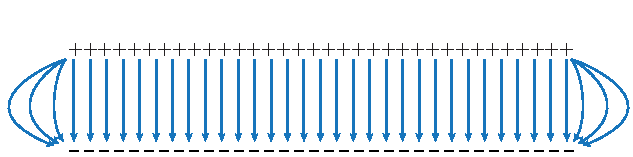
\includegraphics[width=.45\columnwidth]{charge_fields} &
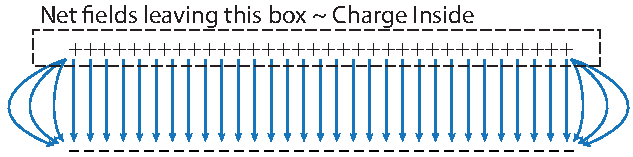
\includegraphics[width=.45\columnwidth]{charge_fields_guass}\\
(a) & (b)\\
\end{tabular}
\caption{(a) Electric field lines leave positive charges and end on negative charges.  (b) If we draw a box around the positive charges, we will find that the net integral of the electric field is positive and outward on the surface of the box.}
\label{fig:mod2-2_ICtech_sld_11}
\end{figure}

\textbf{Gauss’ Law}\index{Gauss' Law} equivalently says that if there is a \textit{net} electric field leaving a region, there has to be positive charge in that region (see \emph{Fig.~\ref{fig:mod2-2_ICtech_sld_11}(b)}).  If we integrate the electric field over a closed surface, then the result will be the net charge inside:
    \begin{align}
    	\oint {\mathcal{E} \cdot dS} &= \frac{Q}{\varepsilon} &\textit{Gauss' Law, closed surface}
    \end{align}
We can derive this from the divergence of charge by integrating over the volume of the closed surface.  Integration of the charge density over the volume is the total charge:
    \begin{equation}
        \oint\limits_V {\nabla \cdot \mathcal{E}\,dV =} \oint\limits_V {\frac{\rho}{\varepsilon}dV = \frac{Q}{\varepsilon}} 
    \end{equation}
The volume integral can be converted into a surface integral using the \textbf{Divergence Theorem}\index{Divergence Theorem}:
    \begin{equation} 
        \oint\limits_V {\nabla \cdot \mathcal{E}\,dV = } \oint\limits_S {\mathcal{E} \cdot dS = } \frac{Q}{\varepsilon}
    \end{equation}
%%%%%%%%%%%%%%%%%%%%%%%%%%%%%%%%%%%%%%%%%%%%
%             SUBSECTION 4.4.2             %
%%%%%%%%%%%%%%%%%%%%%%%%%%%%%%%%%%%%%%%%%%%%
\subsection{Electrostatics in 1D}
Fortunately, most of the problems we will be solving are idealizations in one dimension, and everything simplifies in 1-D.  The divergence operator is a simple derivative:
    \begin{equation} 
        \nabla  \cdot \mathcal{E} = \frac{{d\mathcal{E}}}{{dx}} = \frac{\rho }{\varepsilon } 
    \end{equation}
Which is equivalent to saying that the incremental electrical field is related to an increment of charge:
    \begin{equation} 
        d\mathcal{E} = \frac{\rho }{\varepsilon }dx 
    \end{equation}
If we integrate over the region of interest, we have the total electric field:
    \begin{equation} 
        \mathcal{E}(x) = \mathcal{E}({x_0}) + \int\limits_{{x_0}}^x {\frac{{\rho (x')}}{\varepsilon }} dx'
    \end{equation}
As an application of these equations, one that will become important in the next chapter, consider a uniform charge distribution as shown in \emph{Fig.~\ref{fig:mod2-2_ICtech_sld_13}(a)}.  Integrating the charge density, we get a linear function.  The field increases linearly, as shown in \emph{Fig.~\ref{fig:mod2-2_ICtech_sld_13}(b)}.
    \begin{equation} 
        \mathcal{E}(x) = \int\limits_0^x {\frac{{\rho (x')}}{\varepsilon}} dx' = \frac{{{\rho _0}}}{\varepsilon}x 
    \end{equation}
%%%%%%%%%%%%%%%%%%%%%%%%%%%%%%%%%%%%%%%%%%%%
%                 FIGURE                   %
%%%%%%%%%%%%%%%%%%%%%%%%%%%%%%%%%%%%%%%%%%%%
\begin{figure}[tb]
\centering
\begin{tabular}{cc}
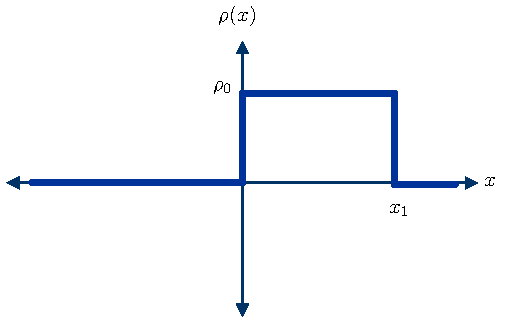
\includegraphics[width=.4\columnwidth]{mod2-2_ICtech_sld_13} &
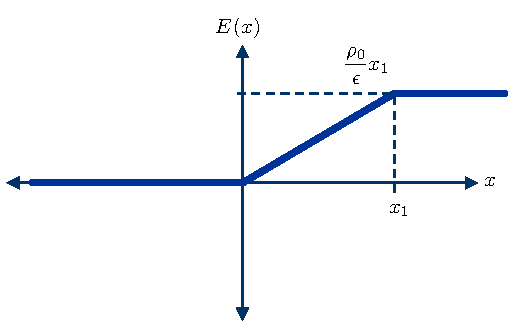
\includegraphics[width=.4\columnwidth]{mod2-2_ICtech_sld_13b}\\
(a) & (b)\\
\end{tabular}
\caption{(a) In this hypothetical example, the charge density is uniform over a region from the origin to $x_1$.  We assume that the field is zero at $x=0$.  (b) Integration of the charge density yields the electric field, which increases linearly up to $x_1$, and remains constant thereafter.} \label{fig:mod2-2_ICtech_sld_13}
\end{figure}
%%%%%%%%%%%%%%%%%%%%%%%%%%%%%%%%%%%%%%%%%%%%
%             SUBSECTION 4.4.3             %
%%%%%%%%%%%%%%%%%%%%%%%%%%%%%%%%%%%%%%%%%%%%
\subsection{Electrostatic Potential}
The electric field (force) is related to the potential (energy):
    \begin{equation} 
        \mathcal{E} =  - \frac{{d\varphi }}{{dx}} 
    \end{equation}
The negative sign says that field lines go from high potential points to lower potential points, and it takes work to push a positive charge against the field:
    \begin{equation} 
        {F_e} = q\mathcal{E} =  - e\frac{{d\varphi }}{{dx}} 
    \end{equation}
Note that as shown in \emph{Fig.~\ref{fig:mod2-2_ICtech_sld_14}(a)}, an electron should “float” to a high potential point since it has negative charge.   
    \begin{equation} 
        \varphi (x) - \varphi ({x_0}) =  - \int_C {\mathcal{E} \cdot d\vec l} 
    \end{equation}
%%%%%%%%%%%%%%%%%%%%%%%%%%%%%%%%%%%%%%%%%%%%
%                 FIGURE                   %
%%%%%%%%%%%%%%%%%%%%%%%%%%%%%%%%%%%%%%%%%%%%
\begin{figure}[H]
\centering
\begin{tabular}{ccc}
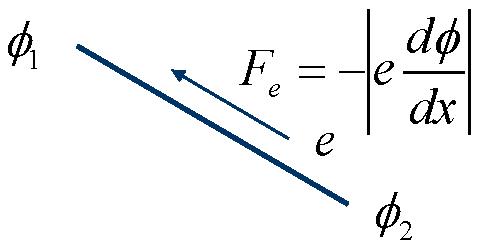
\includegraphics[width=.25\columnwidth]{mod2-2_ICtech_sld_14} &
\hspace{3cm}
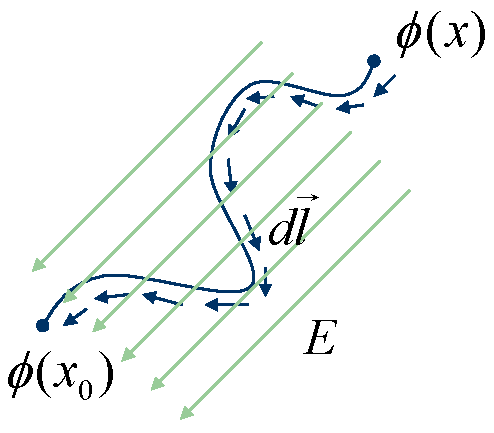
\includegraphics[width=.3\columnwidth]{mod2-2_ICtech_sld_15}\\
(a) & & (b)\\
\end{tabular}
\caption{(a)  The force experienced by an electron is related to the gradient of the potential from point 1 to point 2.  (b)  The work to move a charge against a field is the line integral of the the path over the field, with only paths parallel to the field contributing to the integral.}
\label{fig:mod2-2_ICtech_sld_14}
\end{figure}
%%%%%%%%%%%%%%%%%%%%%%%%%%%%%%%%%%%%%%%%%%%%
The potential is the integral of the field, as shown in \emph{Fig.~\ref{fig:mod2-2_ICtech_sld_14}(b)}.  The integral is path independent for static fields because only the path in the direction of the field contributes, and motion perpendicular to the field does not require any energy expenditure (there are no forces in perpendicular directions).  In one dimension, this is a simple integral:
    \begin{equation} 
        \varphi (x) - \varphi ({x_0}) =  - \int_{{x_0}}^x {\mathcal{E}(x')dx'}  
    \end{equation}
Going the other way, we have Poisson’s equation in 1D:
    \begin{equation} 
        \frac{{{d^2}\varphi (x)}}{{d{x^2}}} =  - \frac{{\rho (x)}}{\varepsilon }
    \end{equation}
%%%%%%%%%%%%%%%%%%%%%%%%%%%%%%%%%%%%%%%%%%%%
%             SUBSECTION 4.4.4             %
%%%%%%%%%%%%%%%%%%%%%%%%%%%%%%%%%%%%%%%%%%%%
\subsection{Boundary Conditions}
Potential must be a continuous function. If not, the fields (forces) would be infinite.  Electric fields need not be continuous. We have already seen that the electric fields diverge on charges. In fact, across an interface shown in \emph{Fig.~\ref{fig:mod2-2_ICtech_sld_16}} we apply Gauss' Theorem: 
    \begin{equation} 
        \oint {\varepsilon \mathcal{E} \cdot dS = - {\varepsilon _1}{\mathcal{E}_1}S + {\varepsilon _2}{\mathcal{E}_2}S = {Q_{inside}}}
    \end{equation}
%%%%%%%%%%%%%%%%%%%%%%%%%%%%%%%%%%%%%%%%%%%%
%                 FIGURE                   %
%%%%%%%%%%%%%%%%%%%%%%%%%%%%%%%%%%%%%%%%%%%%
\begin{figure}[H]
\centering
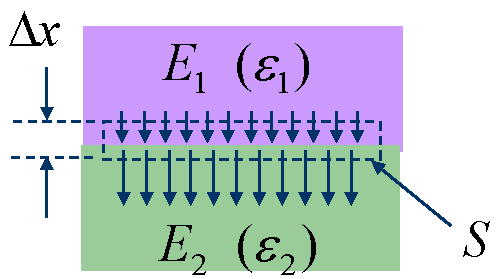
\includegraphics[width=.35\columnwidth]{mod2-2_ICtech_sld_16}
\caption{The boundary conditions at the junction of two materials is determined by applying Guass' Law to a pillbox shaped region surrounding the border, and letting the height of the pillbox $\Delta x$ diminish.}
\label{fig:mod2-2_ICtech_sld_16}
\end{figure}
%%%%%%%%%%%%%%%%%%%%%%%%%%%%%%%%%%%%%%%%%%%%
\noindent
We have assumed that the field is uniform across the interface.  As the "pillbox" around the interface becomes smaller and smaller, the charge inside must be zero:
    \begin{equation} 
        Q_{inside} \xrightarrow[]{\Delta x \rightarrow 0} 0 
    \end{equation}
Simplifying the equations, we have :
    \begin{equation}  
        - {\varepsilon _1}{\mathcal{E}_1}S + {\varepsilon _2}{\mathcal{E}_2}S = 0
    \end{equation}
Or:
    \begin{equation} 
        \frac{{{\mathcal{E}_1}}}{{{\mathcal{E}_2}}} = \frac{{{\varepsilon _2}}}{{{\varepsilon _1}}} 
    \end{equation}
The field is discontinuous across the boundary, which implies charge density at the surface!  The surface charge arises due to the different levels of electric polarization of the dielectric materials (since $\varepsilon$ is different).
\newpage
%%%%%%%%%%%%%%%%%%%%%%%%%%%%%%%%%%%%%%%%%%%%%%%%%%%%%%%%%%%%%%%%%%%%%%%%%%%%%%%%%%%%%%%%
%%%%%%%%%%%%%%%%%%%%%%%%%%%%%%%%%%%%%%%%%%%%%%%%%%%%%%%%%%%%%%%%%%%%%%%%%%%%%%%%%%%%%%%%
%                                   SECTION 4.5                                        %
%%%%%%%%%%%%%%%%%%%%%%%%%%%%%%%%%%%%%%%%%%%%%%%%%%%%%%%%%%%%%%%%%%%%%%%%%%%%%%%%%%%%%%%%
%%%%%%%%%%%%%%%%%%%%%%%%%%%%%%%%%%%%%%%%%%%%%%%%%%%%%%%%%%%%%%%%%%%%%%%%%%%%%%%%%%%%%%%%
\section{IC Capacitors}
%%%%%%%%%%%%%%%%%%%%%%%%%%%%%%%%%%%%%%%%%%%%
%             SUBSECTION 4.5.1             %
%%%%%%%%%%%%%%%%%%%%%%%%%%%%%%%%%%%%%%%%%%%%
\subsection{MIM (Metal-Insulator-Metal) Capacitor}
%%%%%%%%%%%%%%%%%%%%%%%%%%%%%%%%%%%%%%%%%%%%
%                 FIGURE                   %
%%%%%%%%%%%%%%%%%%%%%%%%%%%%%%%%%%%%%%%%%%%%
\begin{figure}[tb]
\centering
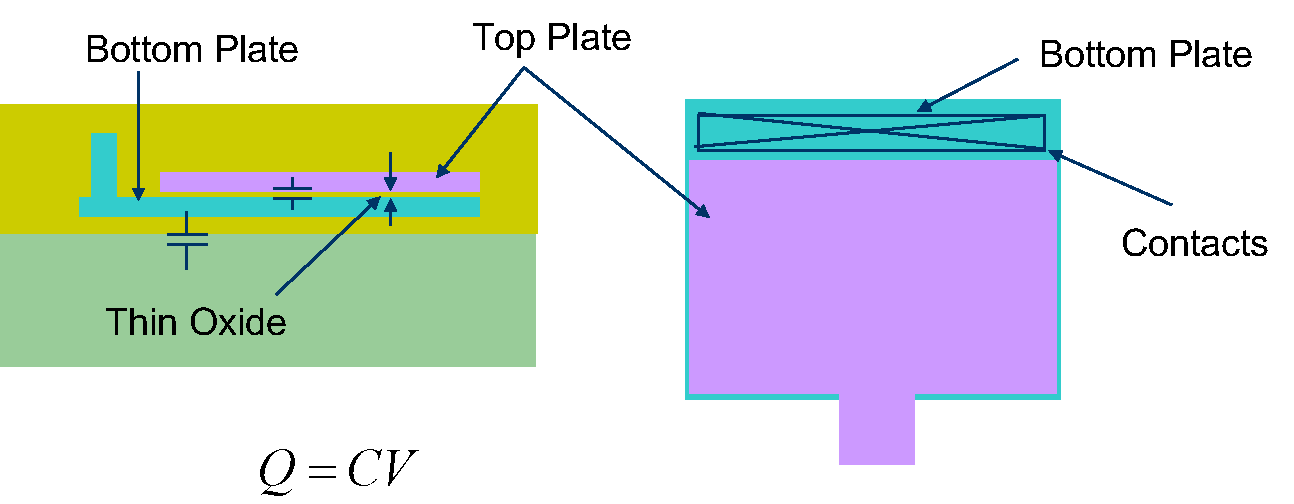
\includegraphics[width=.95\columnwidth]{mod2-2_ICtech_sld_17}
\caption{Integrated circuit capacitors are made by overlapping two large plates, made from interconnect metallization or using polysilicon and doped silicon regions.  The latter types of capacitors are known as MOS capacitors and will be covered in Chapter~\ref{ch:ch07_mos_c}.}
\label{fig:mod2-2_ICtech_sld_17}
\end{figure}
%%%%%%%%%%%%%%%%%%%%%%%%%%%%%%%%%%%%%%%%%%%%
By forming a thin oxide and metal (or polysilicon) plates, an \textbf{MIM capacitor}\index{MIM Capacitor} is formed (\emph{Fig.~\ref{fig:mod2-2_ICtech_sld_17}}).  Metal plates make a higher quality capacitor, but for certain applications, polysilicon gates are sufficient.  Contacts are made to top and bottom plates.  Parasitic capacitance\index{Parasitic capacitance} exists between bottom plate and substrate.
%%%%%%%%%%%%%%%%%%%%%%%%%%%%%%%%%%%%%%%%%%%%
%             SUBSECTION 4.5.2             %
%%%%%%%%%%%%%%%%%%%%%%%%%%%%%%%%%%%%%%%%%%%%
\subsection{Review of Capacitors}
%%%%%%%%%%%%%%%%%%%%%%%%%%%%%%%%%%%%%%%%%%%%
%                 FIGURE                   %
%%%%%%%%%%%%%%%%%%%%%%%%%%%%%%%%%%%%%%%%%%%%
\begin{figure}[tbh]
\centering
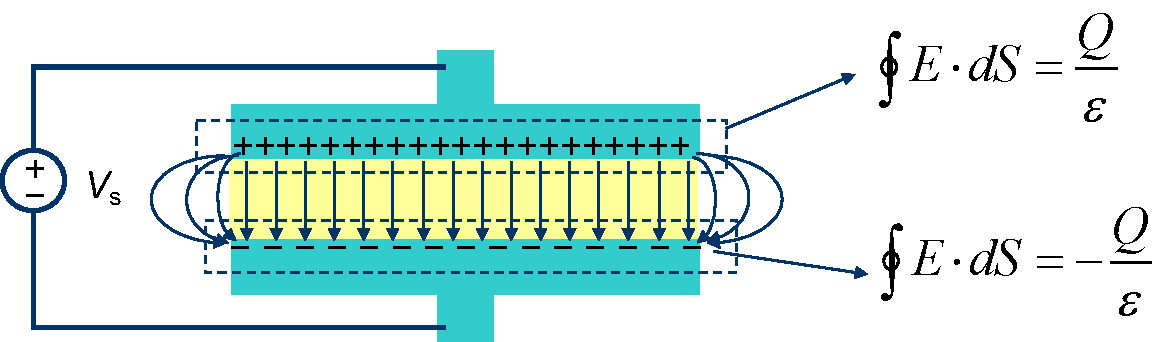
\includegraphics[width=.95\columnwidth]{mod2-2_ICtech_sld_18}
\caption{The charges on a parallel plate capacitor are necessarily equal since the region between the plates is devoid of charge (insulator).}
\label{fig:mod2-2_ICtech_sld_18}
\end{figure}
%%%%%%%%%%%%%%%%%%%%%%%%%%%%%%%%%%%%%%%%%%%%
Armed with electrostatics, we can analyze capacitors in detail.  For example, it is easy to show that the charge on the top and bottom plate are equal (see \emph{Fig.~\ref{fig:mod2-2_ICtech_sld_18}}).  This is true since the field is uniform in the charge free insulator, thus the same fields that leave the top plate must enter the bottom plate.

If we integrate the field from the bottom plate to the top plate, we obtain the applied voltage on the capacitor.  The field is constant, so we have:
    \begin{equation} 
        \int {\mathcal{E} \cdot dl} = {\mathcal{E}_0}\,t_{ox} = V_s \xrightarrow{\hspace*{1cm}}{\mathcal{E}_0} = \frac{V_s}{t_{ox}} 
    \end{equation}
By Gauss' Law, we can relate the field to the charge on the plate:
    \begin{equation} 
        \oint {\mathcal{E} \cdot dS} = {\mathcal{E}_0}\,A = \frac{Q}{\varepsilon} \xrightarrow{\hspace*{1cm}}
        \frac{{{V_s}}}{{{t_{ox}}}}A = \frac{Q}{\varepsilon } \xrightarrow{\hspace*{1cm}}
        Q = C{V_s}
    \end{equation}
\newpage
\noindent
%%%%%%%%%%%%%%%%%%%%%%%%%%%%%%%%%%%%%%%%%%%%
%                 FIGURE                   %
%%%%%%%%%%%%%%%%%%%%%%%%%%%%%%%%%%%%%%%%%%%%
\begin{figure}[tb]
\centering
\begin{tabular}{cc}
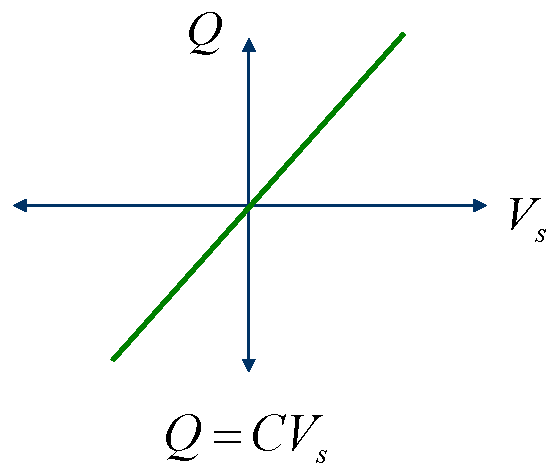
\includegraphics[width=.35\columnwidth]{mod2-2_ICtech_sld_19} &
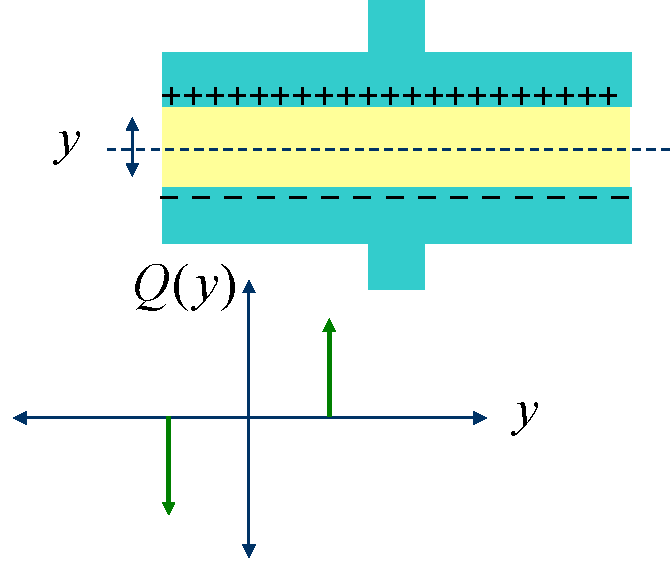
\includegraphics[width=.35\columnwidth]{mod2-2_ICtech_sld_19b}\\
(a) & (b)\\
\end{tabular}
\caption{(a) An ideal capacitor constructed with perfect metals has a linear $Q$-$V$ relation and (b) all the charges reside at the surface of the plates.}
\label{fig:mod2-2_ICtech_sld_19}
\end{figure}
%%%%%%%%%%%%%%%%%%%%%%%%%%%%%%%%%%%%%%%%%%%%
This leads to the well known charge-voltage relationship shown in \emph{Fig.~\ref{fig:mod2-2_ICtech_sld_19}(a)}:
    \begin{align} 
        C &= \frac{A\,\varepsilon}{t_{ox}} &\textit{Capacitance between two parallel plates}
    \end{align}
For an ideal capacitor constructed with metal plates, all charge must be at surface of the plates.  Recall that the field inside of an ideal metal is zero, so that means all the charge is at the surface.  If we plot the charge as a function of position, then we obtain two delta functions, because of the infinite concentration of charge \big(see \emph{Fig.~\ref{fig:mod2-2_ICtech_sld_19}(b)}\big).
%%%%%%%%%%%%%%%%%%%%%%%%%%%%%%%%%%%%%%%%%%%%
%                 FIGURE                   %
%%%%%%%%%%%%%%%%%%%%%%%%%%%%%%%%%%%%%%%%%%%%
\begin{figure}[H]
\centering
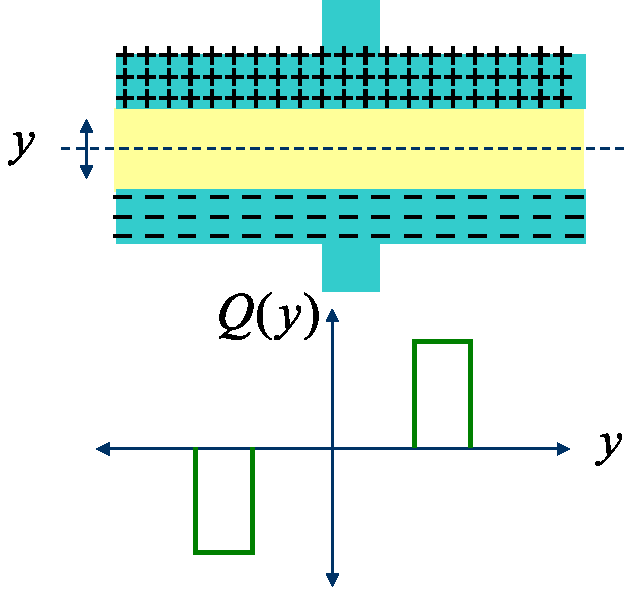
\includegraphics[width=.5\columnwidth]{mod2-2_ICtech_sld_20b} 
\caption{A capacitor structure whereby the charges are distributed uniformly along the plates, something similar to the depletion region that we will study in the next chapter.}
\label{fig:mod2-2_ICtech_sld_20b}
\end{figure}
%%%%%%%%%%%%%%%%%%%%%%%%%%%%%%%%%%%%%%%%%%%%
%%%%%%%%%%%%%%%%%%%%%%%%%%%%%%%%%%%%%%%%%%%%
%             SUBSECTION 4.5.3             %
%%%%%%%%%%%%%%%%%%%%%%%%%%%%%%%%%%%%%%%%%%%%
\subsection{A Non-Linear Capacitor}
We will soon meet capacitors that have a non-linear Q-V relationship.  If plates are not ideal metal, the charge density can penetrate into surface.  For example, suppose the charge is uniformly distributed through the thickness of the plates as shown in \emph{Fig.~\ref{fig:mod2-2_ICtech_sld_20b}}.
%%%%%%%%%%%%%%%%%%%%%%%%%%%%%%%%%%%%%%%%%%%%
For a \textbf{non-linear capacitor}\index{Capacitors!non-linear}, we have a general relationship between the charge and the voltage (see \emph{Fig.~\ref{fig:mod2-2_ICtech_sld_20}}):
    \begin{equation} 
        Q = f({V_s}) \ne C{V_s} 
    \end{equation}
We can’t identify a capacitance like a linear $Q-V$ capacitor.  But now imagine that we apply a small signal on top of a bias voltage.  If the signal is very small, we can do a Taylor Series expansion\index{Taylor expansion}:
    \begin{equation} 
        Q = f({V_s} + {v_s}) \approx f({V_s}) + {\left. {\frac{{df(V)}}{{dV}}} \right|_{V = {V_s}}} \cdot {v_s} 
    \end{equation}
$f(V_s)$ is a constant amount of charge.  The incremental charge is therefore:
    \begin{equation} 
        Q = {Q_0} + q \approx f({V_s}) + {\left. {\frac{{df(V)}}{{dV}}} \right|_{V = {V_s}}} \cdot {v_s}
    \end{equation}
%%%%%%%%%%%%%%%%%%%%%%%%%%%%%%%%%%%%%%%%%%%%
%                 FIGURE                   %
%%%%%%%%%%%%%%%%%%%%%%%%%%%%%%%%%%%%%%%%%%%%
\begin{figure}[tb]
\centering
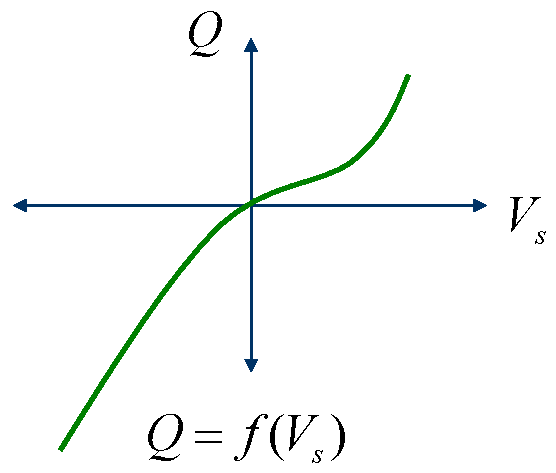
\includegraphics[width=.35\columnwidth]{mod2-2_ICtech_sld_20} 
\caption{A hypothetical non-linear capacitor as is defined by its $Q = f(V)$ relation.} \label{fig:mod2-2_ICtech_sld_20}
\end{figure}
%%%%%%%%%%%%%%%%%%%%%%%%%%%%%%%%%%%%%%%%%%%%
%             SUBSECTION 4.5.4             %
%%%%%%%%%%%%%%%%%%%%%%%%%%%%%%%%%%%%%%%%%%%%
\subsection{Small Signal Capacitance}
To find the \textbf{"small-signal capacitance"}\index{Small-signal capacitance}, break the equation for total charge into two terms:
    \begin{equation} 
        Q = {Q_0} + q \approx f({V_s}) + {\left. {\frac{{df(V)}}{{dV}}} \right|_{V = {V_s}}}{v_s} 
    \end{equation}
    \begin{equation} 
        q = {\left. {\frac{{df(V)}}{{dV}}} \right|_{V = {V_s}}}{v_s} = C\,{v_s} 
    \end{equation}
    \begin{equation} 
        C \equiv {\left. {\frac{{df(V)}}{{dV}}} \right|_{V = {V_s}}} 
    \end{equation}
%%%%%%%%%%%%%%%%%%%%%%%%%%%%%%%%%%%%%%%%%%%%
%             SUBSECTION 4.5.5             %
%%%%%%%%%%%%%%%%%%%%%%%%%%%%%%%%%%%%%%%%%%%%
\subsection{Example of Non-Linear Capacitor}
We will see that for a \emph{PN}-junction, the charge is a function of the reverse bias\index{Reverse bias}:
    \begin{equation} 
        {Q_j}(V) =  - q{N_A}{x_p}\sqrt {1 - \frac{V}{{{\varphi _b}}}} 
    \end{equation}
The small signal capacitance is therefore given by:
    \begin{equation} 
        {C_j}(V) = \frac{{dQ_j^{}}}{{dV}} = \frac{{q{N_A}{x_p}}}{{2{\varphi _b}}}\frac{1}{{\sqrt {1 - \frac{V}{{{\varphi _b}}}}}} = \frac{{C_{j0}^{}}}{{\sqrt {1 - \frac{V}{{{\varphi _b}}}}}} 
    \end{equation}
